\documentclass{article} % Define la clase del documento, en este caso, un artículo
\usepackage[letterpaper,margin=3cm]{geometry} % Configura el tamaño del papel y los márgenes del documento
\usepackage{graphicx} % Permite la inserción de imágenes
\usepackage[spanish]{babel}% Activar esta configuración para informes en español, ajusta el idioma del documento
\usepackage[usenames]{color} % Permite el uso de colores definidos por nombre en el documento
\usepackage{hyperref} % Habilita enlaces y referencias dentro del documento
\hypersetup{colorlinks=true, linkcolor = black, citecolor= black} % Configura el color de los enlaces y citas
\usepackage{booktabs} % Proporciona comandos para crear tablas de alta calidad
\usepackage{natbib} % Permite el uso de citas y referencias bibliográficas con diferentes estilos
\usepackage{tikz} % Permite la creación de gráficos y diagramas vectoriales directamente en LaTeX
\usepackage{float} % Para controlar la posición de los elementos flotantes, como imágenes, con la opción [H]
\usepackage{diagbox} % Permite crear celdas con líneas diagonales en tablas
\usepackage{listings} % Permite la inclusión y formateo de código fuente en el documento
\usepackage{xcolor} % Paquete para definir y usar colores en el documento
\usepackage{parskip} % Añade espacio entre párrafos en lugar de sangrías
\usepackage{fancyhdr} % Permite personalizar encabezados y pies de página
\usepackage{amsmath} % Proporciona una amplia variedad de entornos y comandos matemáticos

\pagestyle{fancy} % Usa el estilo fancyhdr
\fancyhf{} % Borra todos los encabezados y pies de página
\renewcommand{\headrulewidth}{0pt}
\renewcommand{\footrulewidth}{0pt} % Desactiva la línea horizontal predeterminada en el pie
\setlength{\headheight}{2cm} % Ajusta la altura del encabezado para hacer espacio para la línea
\fancyhead[L]{\raisebox{0.20cm}{\textbf{Proyecto de infraestructura hidráulica}}} % Añade el texto en la parte izquierda del encabezado, subiéndolo ligeramente
\fancyhead[R]{\raisebox{0.1cm}{
\includegraphics[width=0.25\linewidth]{LOGO_UNIVERSIDAD.jpg}}} % Añade la imagen en la parte derecha del encabezado y súbela un poco
\fancyhead[C]{\rule{\textwidth}{0.6pt}} % Añade una línea horizontal superior centrada
\fancyfoot[C]{\rule{\textwidth}{0.6pt}} % Añade una línea horizontal en el pie de página centrada
\fancyfoot[R]{\raisebox{-1.5\baselineskip}{\thepage}} % Coloca el número de página a la derecha, con suficiente espacio debajo de la línea
\geometry{top=3cm, bottom=2.5cm} % Ajusta los márgenes superior e inferior

% Definición de colores al estilo Visual Studio Code
\definecolor{codegreen}{rgb}{0.25,0.49,0.48} % Comentarios
\definecolor{codegray}{rgb}{0.5,0.5,0.5} % Números y anotaciones
\definecolor{codepurple}{rgb}{0.58,0,0.82} % Palabras clave
\definecolor{backcolour}{rgb}{0.95,0.95,0.92} % Color de fondo

% Configuración del estilo de las celdas de código
\lstset{
    backgroundcolor=\color{backcolour},   % color de fondo; necesita que el paquete color o xcolor esté cargado
    commentstyle=\color{codegreen},       % estilo de comentarios
    keywordstyle=\color{codepurple},      % estilo de palabras clave
    numberstyle=\tiny\color{codegray},    % estilo de los números de línea
    stringstyle=\color{red},              % estilo de las cadenas de texto
    basicstyle=\ttfamily\small,           % estilo del texto básico
    breakatwhitespace=false,              % ajustes de líneas sólo en espacios en blanco
    breaklines=true,                      % ajustar las líneas si son muy largas
    captionpos=b,                         % posición de la leyenda (abajo)
    keepspaces=true,                      % preserva los espacios en el texto; útil si se usa monoespaciado
    numbers=left,                         % dónde poner los números de línea
    numbersep=5pt,                        % qué tan lejos están los números de línea del código
    showspaces=false,                     % mostrar espacios con subrayados particulares; reemplaza 'showstringspaces'
    showstringspaces=false,               % subrayar los espacios dentro de las cadenas solo
    showtabs=false,                       % mostrar tabulaciones en el código con subrayados particulares
    tabsize=2,                            % tamaños de tabulación a 2 espacios
    language=TeX,                         % lenguaje del código
    morecomment=[l]\#,                    % reconocer # como inicio de comentario en Python
    frame=single,                         % agregar un marco simple alrededor del código
    rulecolor=\color{black}               % color del marco
}

\begin{document}
%----------------------------------------------------------------------------------------
%   PORTADA
%Modificar desde aqui en adelante
%----------------------------------------------------------------------------------------
\begin{titlepage}%Inicio de la carátula, solo modificar los datos necesarios
\newcommand{\HRule}{\rule{\linewidth}{0.5mm}} 
\center 
%----------------------------------------------------------------------------------------
%	ENCABEZADO
%----------------------------------------------------------------------------------------

\includegraphics[width=10cm]{LOGO_UNIVERSIDAD.jpg}\\ % Si esta plantilla se copio correctamente, va a llevar la imagen del logo de la facultad.OBS: Es necesario incluir el paquete: graphicx
\vspace{3cm}
%----------------------------------------------------------------------------------------
%	SECCION DEL TITULO
%----------------------------------------------------------------------------------------
\HRule \\[0.4cm]
{ \huge \bfseries Caso 2: Infraestructura en Recursos Hídricos}\\[0.4cm] % Titulo del documento
{ \huge \bfseries Proyecto de Infraestructura Hidráulica}\\[0.4cm] % Titulo del documento
\HRule \\[1.5cm]
 \vspace{5cm}
%----------------------------------------------------------------------------------------
%	SECCION DEL AUTOR
%----------------------------------------------------------------------------------------
\begin{flushright}
    { \textbf{Profesor:}\\
    Oscar Loyola\\
    \vspace{0.2cm}
    \textbf{Alumnos:}\\
    Bernardo Caprile Canala-Echevarría\\
    Pedro Valenzuela Béjares\\
    Francisco Zegers
    \vspace{0.2cm}

}
\end{flushright}
\vspace{1cm}
%----------------------------------------------------------------------------------------
%	SECCION DE LA FECHA
%----------------------------------------------------------------------------------------
{\large \textbf{\today}}\\[2cm] % El comando \today coloca la fecha del dia, y esto se actualiza con cada compilacion, en caso de querer tener una fecha estatica, reemplazar el \today por la fecha deseada
\end{titlepage}
%----------------------------------------------------------------------------------------
%  INDICE
%----------------------------------------------------------------------------------------
\newpage
\section*{Resumen Ejecutivo}

El presente informe describe el diseño de una obra de captación y una barrera de derivación en el río Pilmaiquén, cuyo propósito es abastecer una planta de agua potable mediante la captación controlada de un caudal de 10\,m³/s. El proyecto considera criterios hidráulicos, estructurales y geotécnicos que aseguran una operación continua, segura y eficiente frente a condiciones normales y de crecida.

La obra propuesta se compone de una barrera mixta de 130\,m de longitud, constituida por un módulo de compuertas en concreto armado de 30\,m y un tramo de tierra compactada de 100\,m. El sistema incorpora cuatro compuertas de 5\,m de ancho y 8\,m de alto, separadas por machones de 1\,m, que permiten un control eficaz del caudal y una respuesta estable ante crecidas con períodos de retorno de 250 y 500 años.

El análisis hidráulico se desarrolló mediante modelaciones en el software HEC-RAS, utilizando información topográfica del cauce y considerando los caudales asociados a los distintos escenarios de operación. Los resultados demostraron que la estructura mantiene un comportamiento estable, evitando el sobrepaso y garantizando el control del flujo en todas las condiciones analizadas. La altura crítica determinada (\(B_c = 7{,}4\,\text{m}\)) fue el parámetro controlador para el dimensionamiento de las compuertas, a las que se adicionó una revancha de seguridad.

Desde el punto de vista geotécnico, se establecieron taludes de 3H:1V aguas arriba y 2{,}5H:1V aguas abajo, coherentes con los materiales presentes en el sitio y con factores de seguridad superiores a los mínimos exigidos. La solución mixta adoptada combina durabilidad y economía, aprovechando las ventajas del concreto armado en la zona de mayor solicitación y del material compactado en los sectores restantes.

En síntesis, la propuesta desarrollada cumple con los criterios técnicos y normativos para obras de \textit{Categoría A}, proporcionando una infraestructura robusta, eficiente y ambientalmente compatible, que asegura el aprovechamiento sostenible de los recursos hídricos del río Pilmaiquén.

\newpage
\tableofcontents % Genera el índice automáticamente
\newpage
\section{Introducción}

El presente informe expone el diseño de una obra de captación y una barrera de derivación destinadas a abastecer una planta de agua potable mediante la captación controlada de un caudal de 10 m³/s proveniente del río Pilmaiquén. El objetivo principal es desarrollar una infraestructura capaz de garantizar un flujo continuo, estable y seguro, incluso bajo condiciones de crecida, manteniendo una operación eficiente y confiable.

El estudio considera el análisis hidrológico e hidráulico del río en el sector de la bocatoma, así como la evaluación geotécnica del terreno, compuesto principalmente por depósitos fluviales de gravas, gravillas y arenas de baja compactación. Estos antecedentes fueron la base para definir los criterios de diseño estructural e hidráulico de la obra, asegurando su estabilidad y desempeño frente a las solicitaciones de operación y eventos extremos.

El diseño contempla una barrera mixta, conformada por concreto armado en la zona donde se ubican las compuertas para resistir mayores esfuerzos hidráulicos y material de tierra compactada en los sectores restantes, con el fin de optimizar recursos y adaptarse a las condiciones topográficas del sitio. La estructura incluye cuatro compuertas de 5 metros de ancho y 8 metros de altura, separadas por machones de 1 metro, que permiten un control eficiente del caudal y una respuesta adecuada frente a crecidas de hasta 500 años de período de retorno.

El desarrollo de este informe presenta los criterios adoptados, los procedimientos de cálculo y los resultados obtenidos, los cuales sustentan la propuesta de diseño final de la obra. Este trabajo busca aportar una solución técnicamente sólida y ambientalmente compatible, que permita aprovechar de manera eficiente los recursos hídricos del río Pilmaiquén garantizando su operación segura y sostenida en el tiempo.

\newpage
\section{Objetivos y Alcance del Proyecto}

\subsection{Objetivo General}

Diseñar la obra de captación y la barrera de derivación destinadas a una planta de agua potable con un caudal de diseño de 10 m³/s, garantizando una operación segura, continua y eficiente bajo distintas condiciones hidráulicas y estructurales.

\subsection{Objetivos Específicos}

\begin{itemize}
    \item Analizar el régimen hidrológico del río Pilmaiquén en la zona de emplazamiento, considerando caudales de diseño, operación y crecida para distintos períodos de retorno.
    \item Determinar la configuración óptima de la obra de toma y la barrera de derivación, asegurando condiciones adecuadas de captación, sedimentación y control de caudales.
    \item Modelar hidráulicamente el comportamiento del flujo mediante el software HEC-RAS para evaluar la respuesta de la estructura frente a condiciones normales y extremas.
    \item Definir el área mínima del túnel de conducción, considerando la capacidad hidráulica necesaria y las condiciones estructurales del macizo rocoso.
    \item Evaluar las condiciones geotécnicas del sitio para proponer una solución estructural estable y compatible con los materiales existentes.
\end{itemize}

\subsection{Alcance del Proyecto}

El presente proyecto abarca el análisis, diseño y dimensionamiento de los componentes principales de la obra de captación y su infraestructura asociada. Esto incluye el estudio hidrológico e hidráulico del río Pilmaiquén, la definición del emplazamiento del muro y la bocatoma, el diseño de las compuertas, la reja de captación, el túnel de conducción y la barrera mixta de concreto y tierra. Asimismo, se incorporan los criterios de diseño asociados a las crecidas de diseño y verificación correspondientes a una obra de Categoría A, garantizando la funcionalidad y estabilidad del sistema ante condiciones de operación y eventos extremos.

\newpage
\section{Marco Teórico}

El análisis hidráulico de una obra de captación con compuertas requiere determinar el comportamiento del flujo bajo distintas condiciones de operación y crecida. Entre los parámetros fundamentales se encuentra la altura crítica del flujo, representada por \( B_c \), la cual permite establecer la condición de energía mínima en la que el régimen pasa de subcrítico a supercrítico. Este parámetro es clave para el dimensionamiento y la verificación de las compuertas, ya que asegura una operación estable y controlada del sistema de derivación.

\subsection{Determinación de la altura crítica}

La altura crítica del flujo (\( B_c \)) se determina a partir de la relación entre el caudal total, la gravedad y la geometría del canal o estructura. La expresión utilizada para su cálculo es:

\[
B_c = \frac{3}{2 \sqrt[3]{g}} \left( \frac{Q}{b} \right)^{\tfrac{2}{3}}
\]

donde:

\begin{itemize}
    \item \( B_c \): altura crítica del flujo (m),
    \item \( g \): aceleración de gravedad (9,81 m/s²),
    \item \( Q \): caudal que atraviesa las compuertas (m³/s),
    \item \( b \): ancho total efectivo de paso o suma de los anchos de las compuertas abiertas (m).
\end{itemize}

Esta ecuación proviene de la condición de energía específica mínima en canales de sección rectangular. En este punto, la profundidad del flujo (\( B_c \)) se asocia al caudal que puede circular por la compuerta con el menor valor posible de energía específica, garantizando un régimen estable y evitando fenómenos como la formación de resaltes hidráulicos o pérdida de control aguas abajo.

\subsection{Crecidas de diseño y condiciones de operación}

De acuerdo con la normativa hidráulica nacional vigente para obras de captación, evacuación y desagüe particularmente los criterios utilizados por la Dirección General de Aguas (DGA) y las recomendaciones del Manual de Diseño de Obras Hidráulicas, las estructuras se clasifican según su altura y función hidráulica. En este caso, la barrera analizada corresponde a una estructura de \textit{Categoría A}, dado que presenta una altura superior a 5\,m e inferior a 15\,m. Para este tipo de obras, se establecen dos eventos característicos de cálculo: una crecida de diseño con período de retorno de 250 años, utilizada para el dimensionamiento hidráulico y estructural ordinario, y una crecida de verificación con período de retorno de 500 años, destinada a evaluar el comportamiento de la obra frente a condiciones extremas y garantizar su estabilidad global.

El análisis hidráulico se desarrolló considerando dos configuraciones de operación de las compuertas. En la condición de diseño, se asumió que un 25\,\% de las compuertas permanece cerrada mientras el resto opera normalmente, representando la situación típica de regulación del caudal derivado hacia la planta. En la condición de verificación, en cambio, se consideró la apertura total de las compuertas, lo que permite evacuar el caudal máximo posible durante un evento extraordinario y evitar el sobrepaso del muro. La comparación de ambos escenarios permite confirmar que la obra opera en régimen estable y seguro bajo condiciones normales y de crecida, cumpliendo con las exigencias establecidas para obras hidráulicas de esta categoría.

\subsection*{Coeficiente de Manning}

El coeficiente de Manning, denotado como $n$, es un parámetro empírico utilizado en la ecuación de Manning para describir la resistencia al flujo en canales abiertos. Representa los efectos combinados de la rugosidad superficial, irregularidades, vegetación, alineación y variaciones en la sección transversal del canal sobre la pérdida de energía por fricción.

El valor de $n$ depende del material y de las condiciones del canal; por ejemplo, canales de concreto liso presentan valores de $n$ cercanos a 0.012, mientras que cauces naturales con vegetación o irregularidades pueden tener valores superiores a 0.035.


\newpage
\section{Desarrollo}

A partir de los procedimientos descritos en las secciones anteriores, se obtuvieron los principales resultados hidráulicos y geométricos de la obra de captación y su sistema de compuertas. El análisis consideró las condiciones de diseño y verificación establecidas para una obra de Categoría A, según los períodos de retorno definidos de 250 y 500 años, respectivamente.

\subsection{Altura crítica del flujo}

Aplicando la expresión para la altura crítica del flujo presentada en el marco teórico, se determinaron los valores correspondientes a las condiciones de diseño (con un 25\% de compuertas cerradas) y de verificación (todas las compuertas abiertas). Los resultados se resumen en la Tabla~\ref{tab:bcresultados}.

\begin{table}[htbp]
\centering
\begin{tabular}{lcc}
\hline
Condición de operación & Configuración de compuertas & Altura crítica \( B_c \) [m] \\
\hline
Diseño & 25\% cerradas & 7,4 \\
Verificación & Todas abiertas & 5,6 \\
\hline
\end{tabular}
\caption{Alturas críticas del flujo determinadas para las condiciones de diseño y verificación.}
\label{tab:bcresultados}
\end{table}

El criterio de diseño es el que controla el dimensionamiento de las compuertas, ya que presenta la mayor altura crítica. En este caso, la altura de diseño considerada fue de \( B_c = 7{,}4\,\text{m} \), valor que ya incorpora una \textit{revancha} de 1\,m como margen de seguridad sobre el nivel crítico calculado. Este margen permite absorber eventuales incrementos en el nivel del agua debido a turbulencias, obstrucciones parciales o variaciones locales del flujo. Al adoptar finalmente una altura total de compuerta de 8\,m, se obtiene una revancha efectiva de aproximadamente 1{,}6\,m, garantizando la operación segura y estable de la estructura bajo las condiciones más exigentes de diseño.

\subsection{Muro de barrera}

La barrera de derivación presenta una longitud total de 130\,m, medida a lo largo del eje del muro. En la ribera derecha se ubica el tramo construido en concreto armado, que corresponde al módulo donde se disponen las compuertas y los elementos de control hidráulico. El resto de la estructura, hacia la ribera izquierda, se ejecutará en material de tierra compactada, conformando una barrera mixta que combina resistencia estructural y economía constructiva.

El tramo de concreto en ribera derecha tiene una longitud aproximada de 30\,m, suficiente para alojar las cuatro compuertas, los machones intermedios, los estribos laterales y los muros de encauce aguas arriba y aguas abajo. Por su parte, el tramo de tierra compactada abarca los 100\,m restantes, adaptándose a la topografía natural del terreno y asegurando la continuidad del cierre hidráulico.

\begin{table}[htbp]
\centering
\begin{tabular}{lc}
\hline
\textbf{Parámetro} & \textbf{Valor} \\
\hline
Longitud total del muro & 130\,m \\
Longitud del módulo de compuertas (concreto) & 30\,m \\
Longitud del tramo de tierra compactada & 100\,m \\
Altura máxima del muro en su punto más bajo & 14\,m \\
Altura del módulo de compuertas & 8\,m (según criterio de diseño controlador) \\
Talud aguas arriba & 3H:1V \\
Talud aguas abajo & 2{,}5H:1V \\
\hline
\end{tabular}
\caption{Dimensiones principales del muro de la barrera.}
\label{tab:dimensiones_muro}
\end{table}

Los taludes adoptados para el tramo de tierra compactada responden a criterios de estabilidad geotécnica, facilidad constructiva y control de filtraciones. El talud aguas arriba se definió con una pendiente de 3H:1V, lo que proporciona un equilibrio adecuado entre estabilidad y control del gradiente hidráulico durante la operación del embalse. Esta inclinación permite además disponer de una superficie suficientemente suave para aplicar revestimientos o enrocados de protección frente a la erosión o el oleaje.

Por su parte, el talud aguas abajo se estableció con una pendiente algo más empinada, de 2{,}5H:1V, dado que no está sometido a presiones hidrostáticas y su estabilidad depende principalmente del peso propio del material. Esta configuración reduce el volumen total de material de relleno sin comprometer la seguridad de la estructura, manteniendo factores de seguridad típicos superiores a 1{,}5 frente al deslizamiento. Ambas pendientes son coherentes con los valores recomendados para diques de materiales sueltos con alturas del orden de 15\,m y materiales de tipo grava-arcillosa o limo-arenosa compactada.

A modo de resumen, la combinación de un módulo de compuertas en concreto armado con un tramo de tierra compactada permite optimizar los costos constructivos y operativos de la barrera, asegurando al mismo tiempo la estabilidad hidráulica y estructural requerida para una obra de captación de esta naturaleza.

En este caso serán 4 compuertas de 5 m de ancho y 8 m de alto cada una, separadas por machones de 1 m, lo que da un ancho total efectivo de paso de 20 m. Además, el muro tendrá un largo total de 130 m, de los cuales 30 m corresponderán al módulo de compuertas en concreto y 100 m al tramo de tierra compactada.

\subsection{Coeficiente de Manning}

Para poder obtener el coeficiente de Manning, se utilizaron los coeficientes dados en el libro \textit{Roughness Characteristics of Natural Channels} (Barnes). En él se encuentran fotografías de distintos tipos de cauces y se les asigna un coeficiente de rugosidad. A continuación, se muestran las ubicaciones que más se asemejan al cauce del río Pilmaiquén junto con su respectivo coeficiente de Manning.

\begin{table}[h!]
    \centering
    \begin{tabular}{c c}
        \textbf{Ubicación} & \textbf{Coeficiente de Manning} \\
        \hline
        \textit{Clark Fork at St. Regis, Mont} & 0.028 \\ 
        \textit{Columbia River at Vernita, Wash} & 0.025 \\
        \textit{Coeur d'Alene River near Prichard, Idaho} & 0.032 \\\hline
    \end{tabular}
\end{table}

\subsection{Diseño de bocatoma}

El diseño de la obra de toma es una parte importante dentro del proyecto, ya que se encarga de permitir el ingreso controlado del caudal desde el río hacia el túnel de conducción. La bocatoma capta 10 m³/s mediante una compuerta lateral.

En términos generales, la obra de toma se compone de tres elementos principales: la reja frontal, que cumple una función de protección; la compuerta de control, que regula el ingreso de agua y permite el cierre en caso de mantenimiento o emergencias; y el túnel de conducción, que transporta el caudal hacia la conducción principal.

La toma se dispone lateralmente al cauce principal, lo que permite reducir la velocidad de aproximación y minimizar el arrastre de sedimentos. La disposición lateral facilita además el mantenimiento y limpieza, ya que el flujo que ingresa a la toma es más controlado que en una entrada frontal.

En la base de la estructura se incorpora un pequeño canal de aproximación que suaviza la transición entre el flujo libre del río y el flujo dentro del túnel; este sector fue diseñado de modo que el flujo mantenga un régimen subcrítico, lo que reduce las pérdidas por turbulencia y evita cavitación.

Anterior a la compuerta se ubica la reja de protección, la cual fue diseñada considerando bajas velocidades de acercamiento para evitar el arrastre de sólidos y minimizar las pérdidas de carga. El ángulo de inclinación de la reja con respecto al flujo es un factor importante, ya que facilita la autolimpieza y reduce el impacto directo del flujo, lo que prolonga la vida útil y disminuye el riesgo de obstrucción. En este caso, la inclinación elegida permite que los residuos se desplacen hacia la superficie del río, donde pueden ser retirados manual o mecánicamente. 


\begin{table}[h]
    \centering
    \begin{tabular}{c c}
        \textbf{Parámetro} & \textbf{Valor} \\
        \hline
        Caudal de diseño & 10 m$^3$/s \\ 
        Ancho de la reja & 4.0 m \\
        Velocidad en el túnel & 1.00 m/s \\
        Porosidad de la reja & 0.6 \\
        Inclinación de la reja vertical & 35 ° \\ \hline
    \end{tabular}
    \caption{Dimensiones y características principales de la bocatoma}
\end{table}

El área efectiva necesaria para el paso del caudal se determina considerando la velocidad de acercamiento y la porosidad de la reja. De acuerdo con la siguiente ecuación:
\begin{equation}
    Q = V_a \cdot B \cdot H \cdot \phi
\end{equation}

Reemplazando valores y despejando la altura:
\begin{equation}
    H = \frac{Q}{V_a \cdot B \cdot \phi} = \frac{10}{1.00 \cdot 4.0 \cdot 0.6} = 4.17 \ \text{m}
\end{equation}

Por lo tanto, la altura útil de la reja se estima en 4,2 metros, lo que representa la superficie necesaria para permitir el paso del caudal de diseño sin exceder la velocidad de entrada adoptada. Esta altura permite un flujo controlado y garantiza que el nivel del agua en la cámara de captación se mantenga dentro de los márgenes operativos previstos.

\begin{table}[h]
    \centering
    \begin{tabular}{c c}
        \textbf{Parámetro} & \textbf{Valor} \\
        \hline
        Ancho de la reja & 4.0 m \\
        Altura útil de la reja & 4.2 m \\ 
        Espacio entre barras de la reja & 0.1 m \\
        Espesor de las barras & 0.02 m \\
        Ángulo de inclinación & 35 ° \\
        Pérdida de carga en la reja & 0.15 m \\ \hline
    \end{tabular}
    \caption{Dimensiones finales de la bocatoma}
\end{table}

El área frontal total de la reja es de 16 m$^2$, con un área libre efectiva de 9,6 m$^2$ considerando la porosidad del 60\%. El material propuesto es acero galvanizado de alta resistencia a la corrosión, montado sobre un marco de hormigón armado empotrado en la estructura de la toma.

\newpage
\section{Resultados}

Con todos los datos se procedió a ocupar el software HEC-RAS, pero primero se ocuparon los datos topográficos del terreno para obtener los cortes transversales del río y analizar de mejor manera el terreno. Luego, se subió esta información a HEC-RAS, obteniendo lo siguiente:

\begin{figure}[h!]
    \centering
    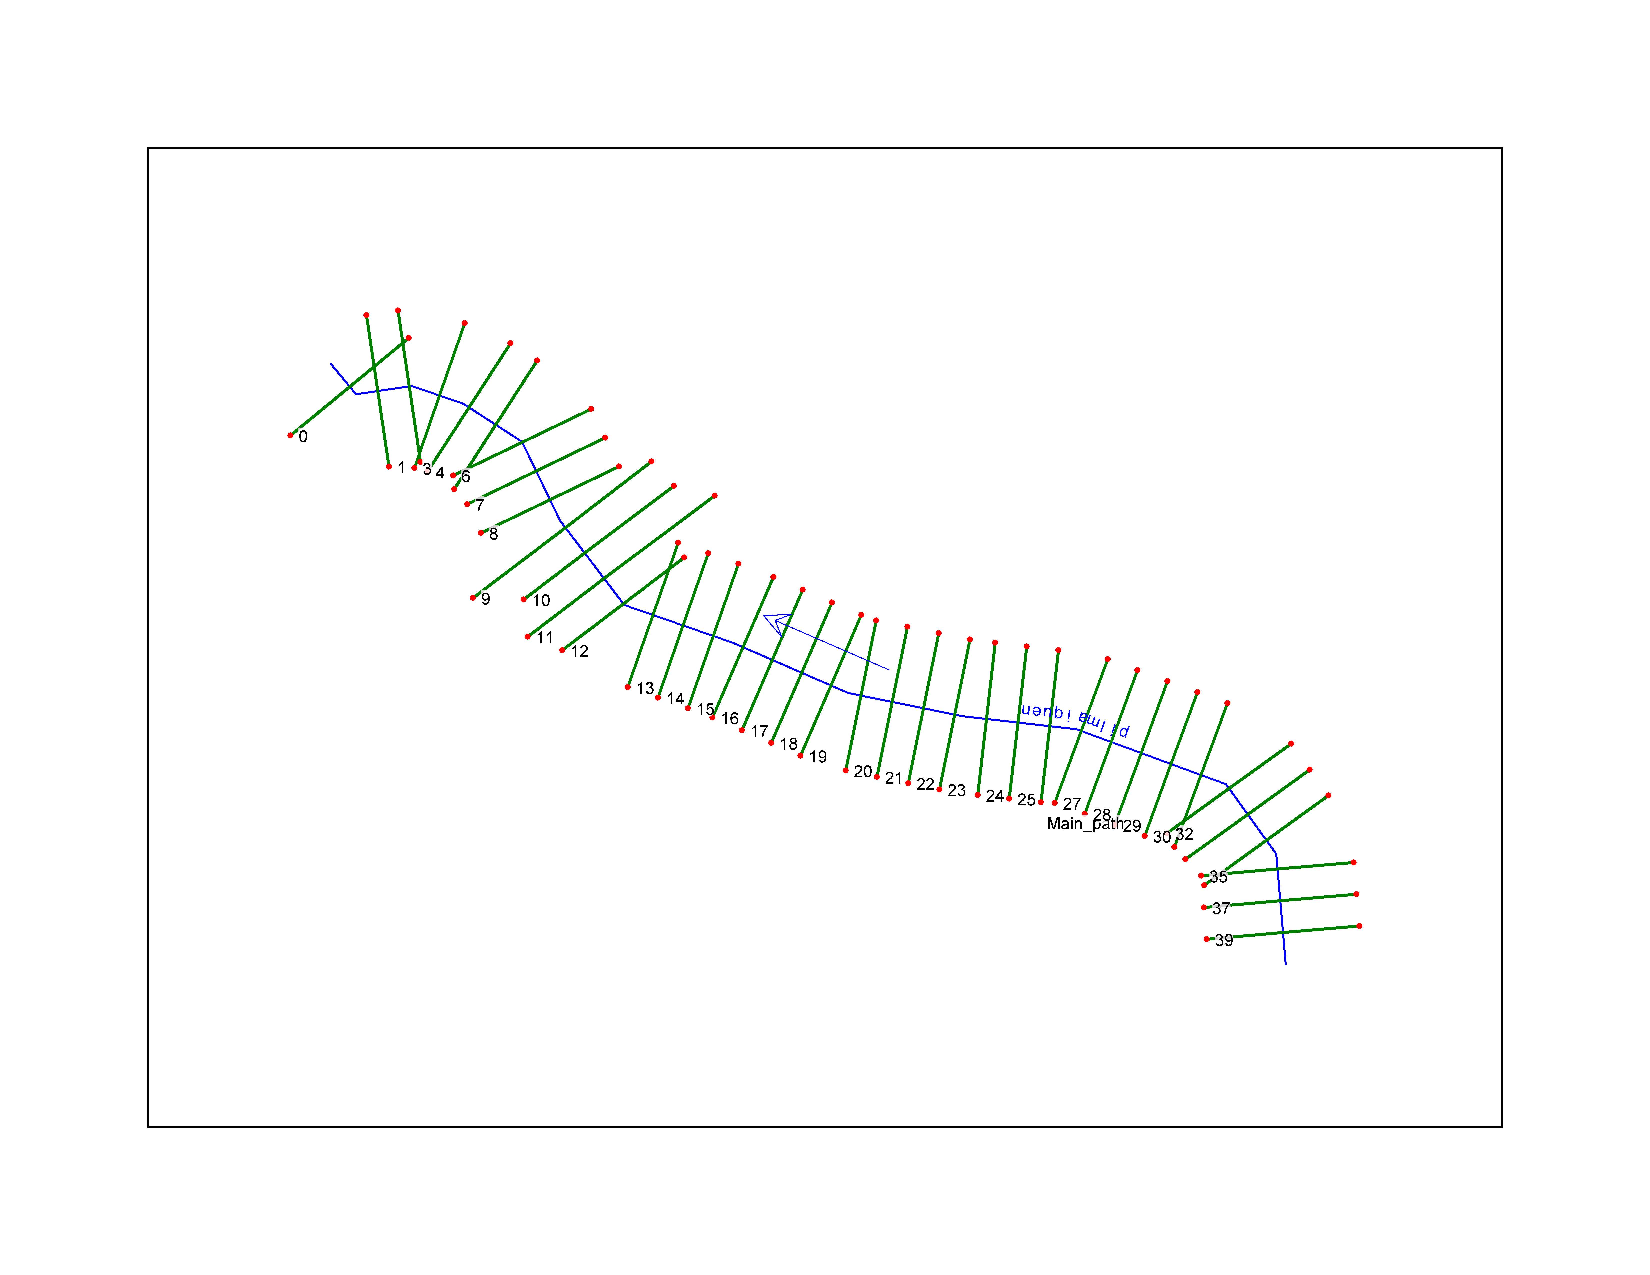
\includegraphics[width=0.6\linewidth]{imagenes/rio_sin_estruc.pdf}
    \caption{Cortes transversales del río Pilmaiquén obtenidos en HEC-RAS}
\end{figure}

Antes de empezar a incorporar al software las bocatomas y el muro, se corrió con los dos caudales asociados a los periodos de retorno de la categoría:

\begin{table}[h]
    \centering
    \begin{tabular}{c c}
        \textbf{Periodo de retorno (años)} & \textbf{Caudal (m$^3$/s)} \\
        \hline
        250 & 396 \\ 
        500 & 418 \\\hline
    \end{tabular}
    \caption{Caudales asociados a los periodos de retorno}
\end{table}

A continuación, se muestran los perfiles hidráulicos con los caudales anteriormente mostrados:

\begin{figure}[H]
    \centering
    \includegraphics[width=0.6\linewidth]{imagenes/perfil_250_sb.pdf}
    \caption{Perfil hidráulico con caudal asociado a periodo de retorno de 250 años}
\end{figure}

\begin{figure}[H]
    \centering
    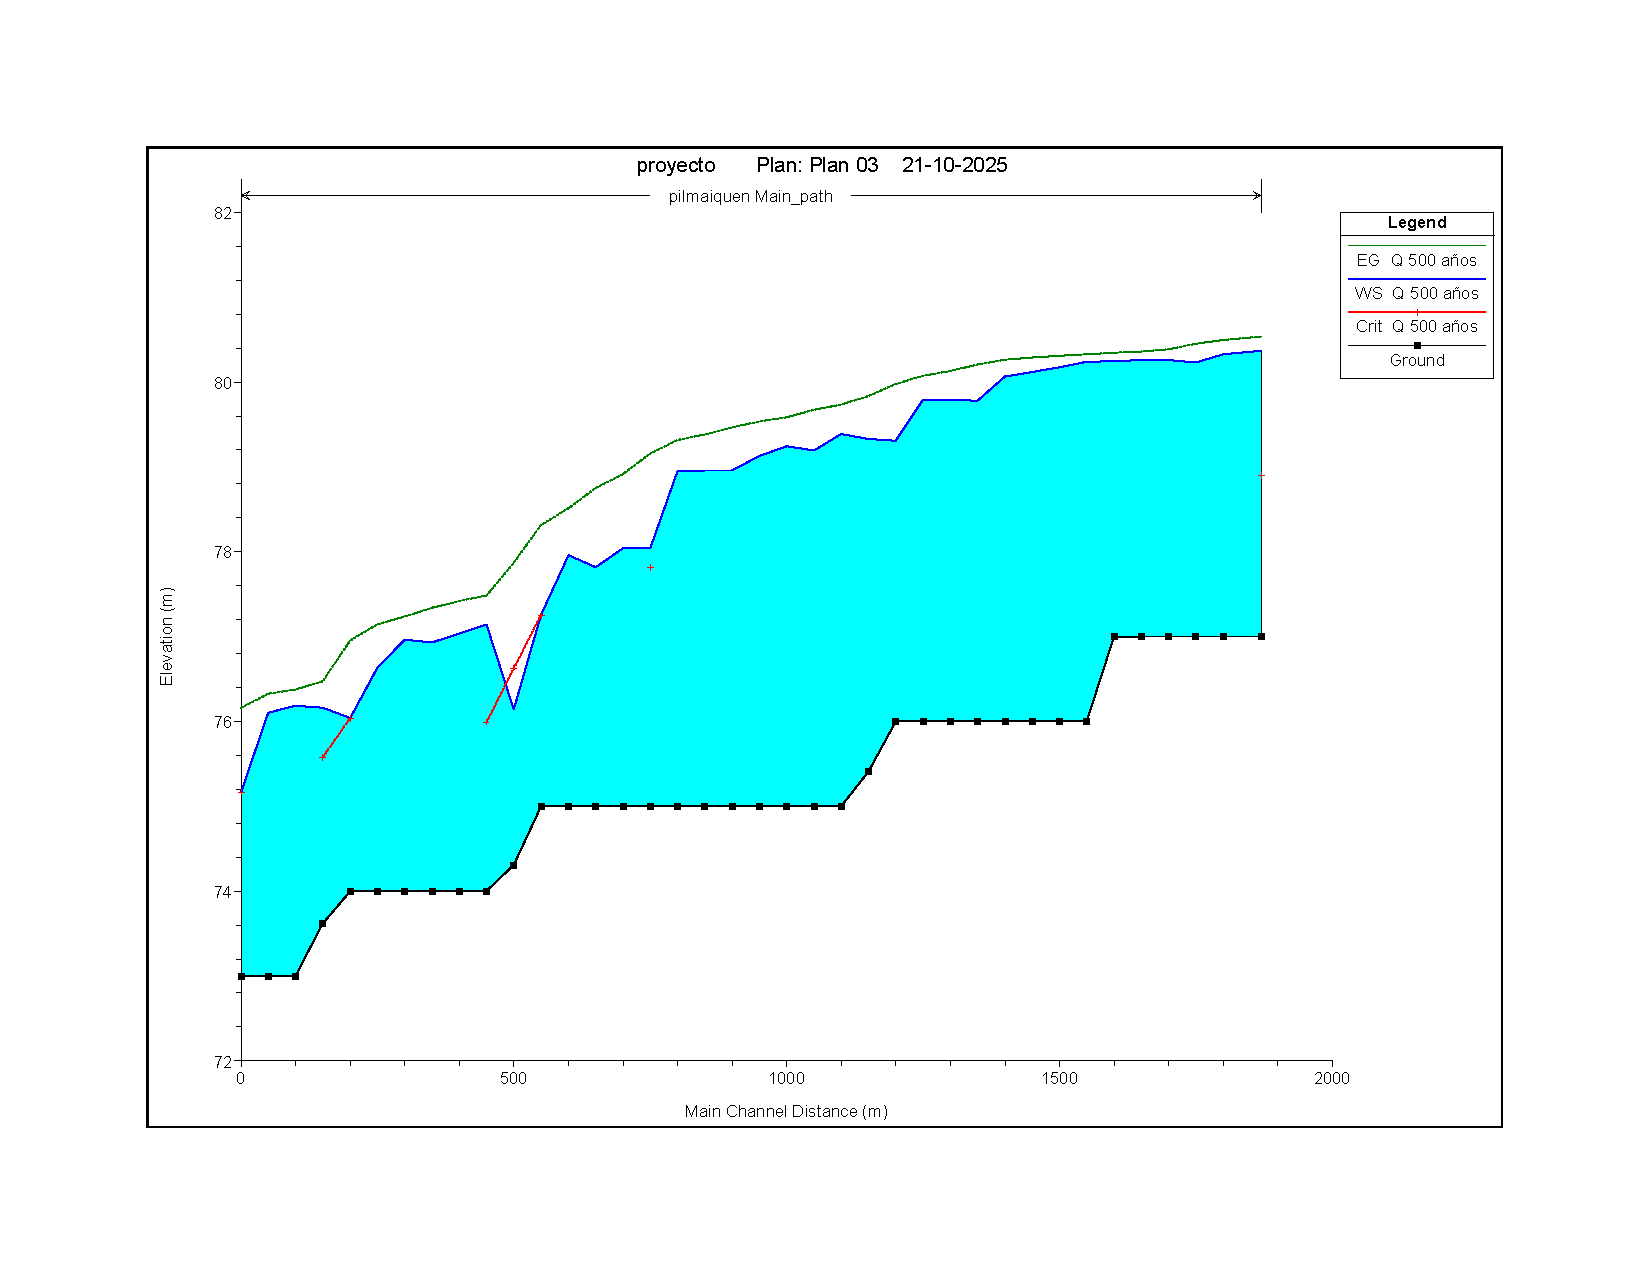
\includegraphics[width=0.6\linewidth]{imagenes/perfil_500_sb.pdf}
    \caption{Perfil hidráulico con caudal asociado a periodo de retorno de 500 años}
\end{figure}

Con los cálculos anteriormente hechos se puede empezar a dimensionar el muro con las compuertas, que se vería de la siguiente manera:

\begin{figure}[H]
    \centering
    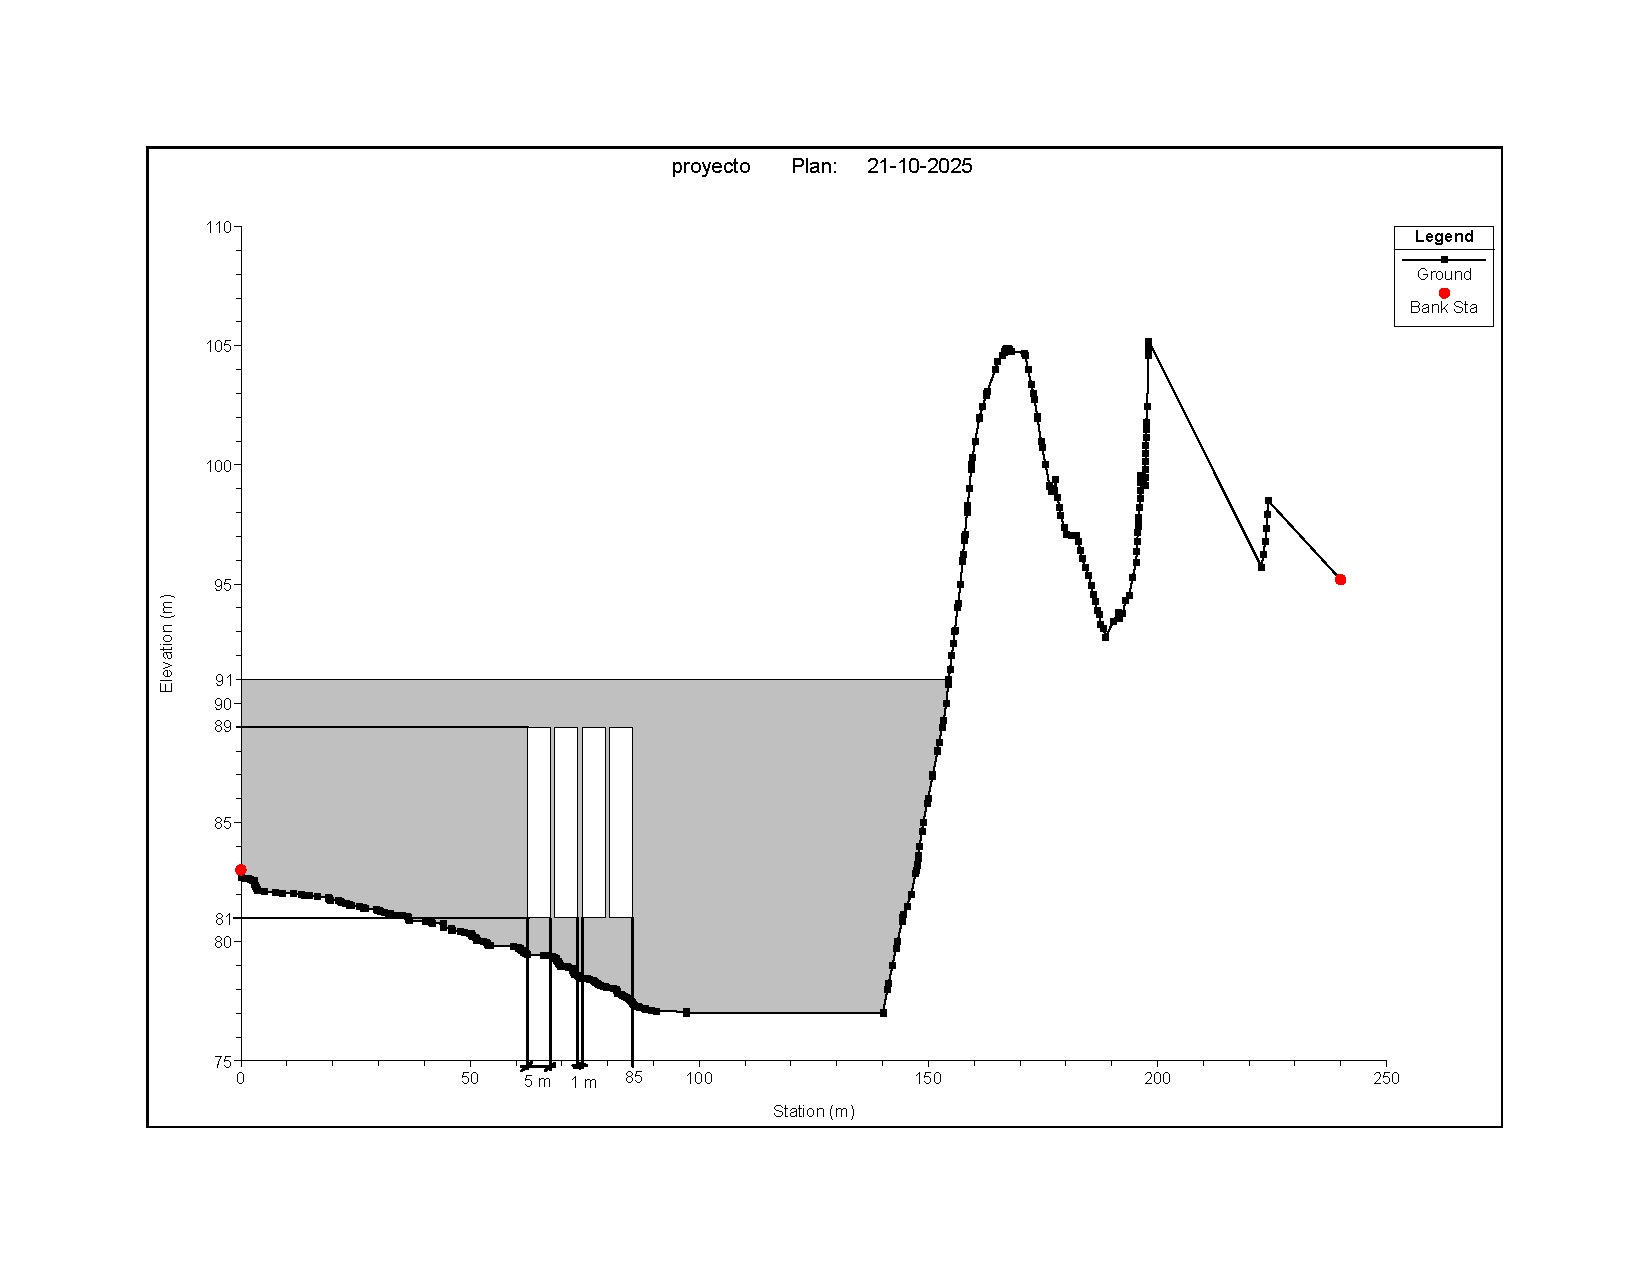
\includegraphics[width=0.8\linewidth]{imagenes/muro.pdf}
    \caption{Muro con bocatomas incorporadas al cauce del río Pilmaiquén}
\end{figure}

En donde sería un muro mixto: desde los 100 metros hacia la ribera derecha del río sería de hormigón, mientras que la otra parte sería un terraplén de tierra compactada.

Luego, ocupando la experiencia de Haber-Maas, se decidió poner el muro al principio de la primera curva; de esta manera la cantidad de sedimento que se va a tener que filtrar y contener será menor. Por lo tanto, la nueva vista de esta sección del río se verá de la siguiente manera:

\begin{figure}[H]
    \centering
    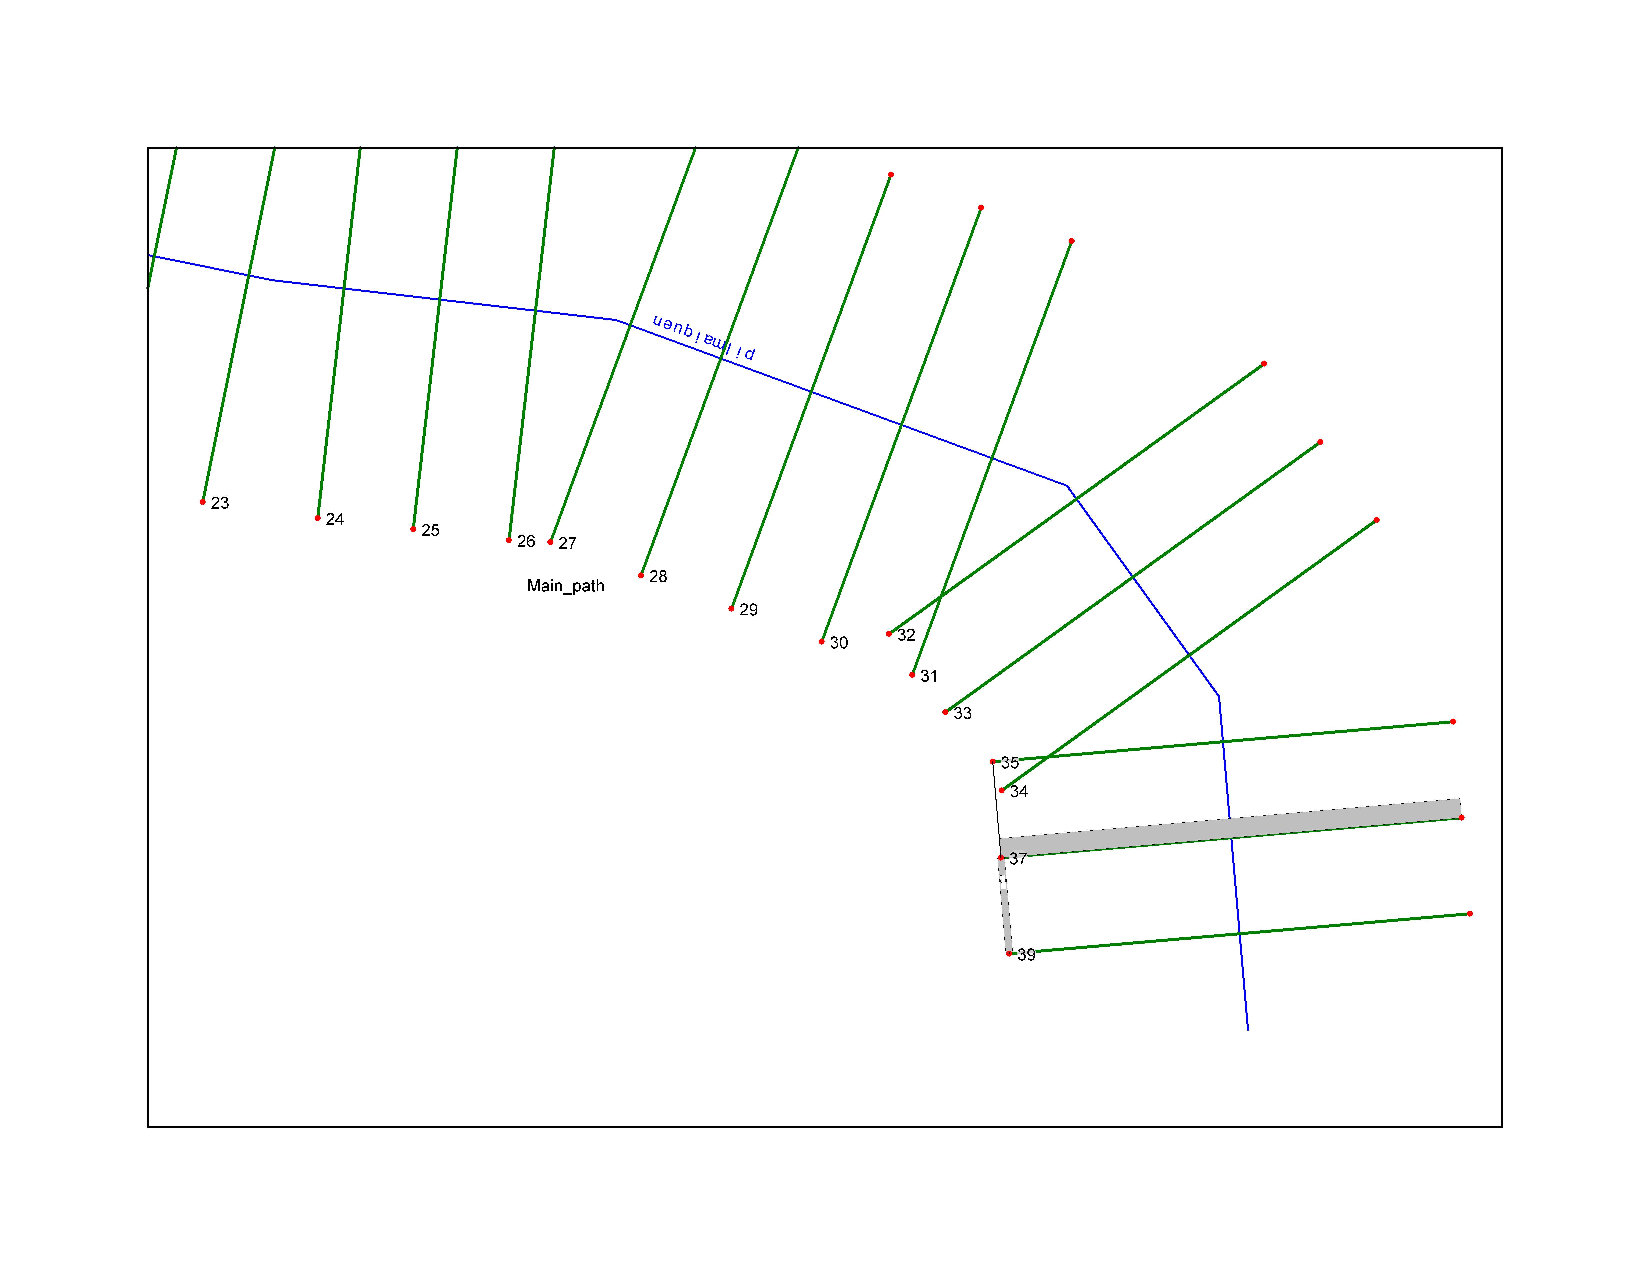
\includegraphics[width=0.6\linewidth]{imagenes/rio.pdf}
    \caption{Cortes transversales del río Pilmaiquén con el muro y las bocatomas incorporadas}
\end{figure}

Una vez lista la geometría, se procedió a correr la simulación con los periodos de retorno anteriormente mencionados, dando los siguientes resultados:

\begin{figure}[H]
    \centering
    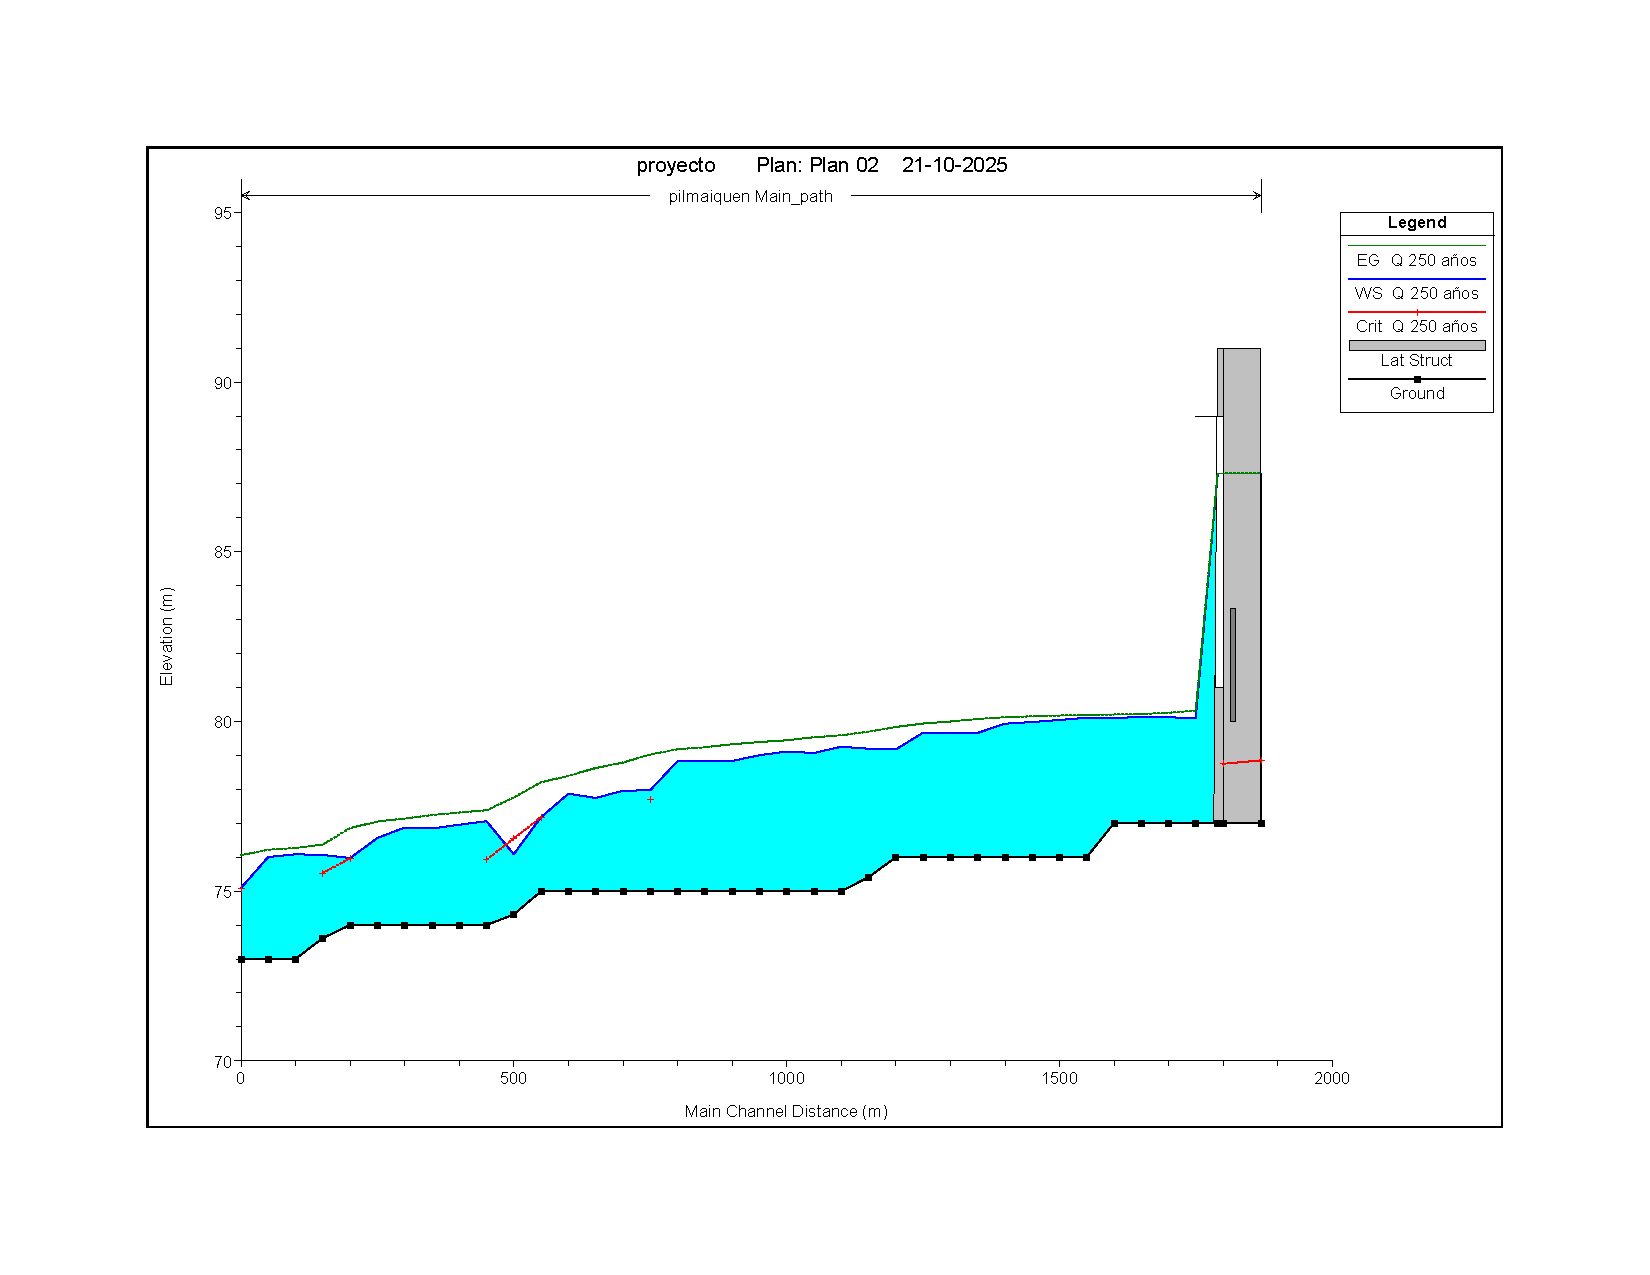
\includegraphics[width=0.6\linewidth]{imagenes/perfil_250_cb.pdf}
    \caption{Perfil hidráulico con caudal asociado a periodo de retorno de 250 años con muro y bocatomas}
\end{figure}

\begin{figure}[H]
    \centering
    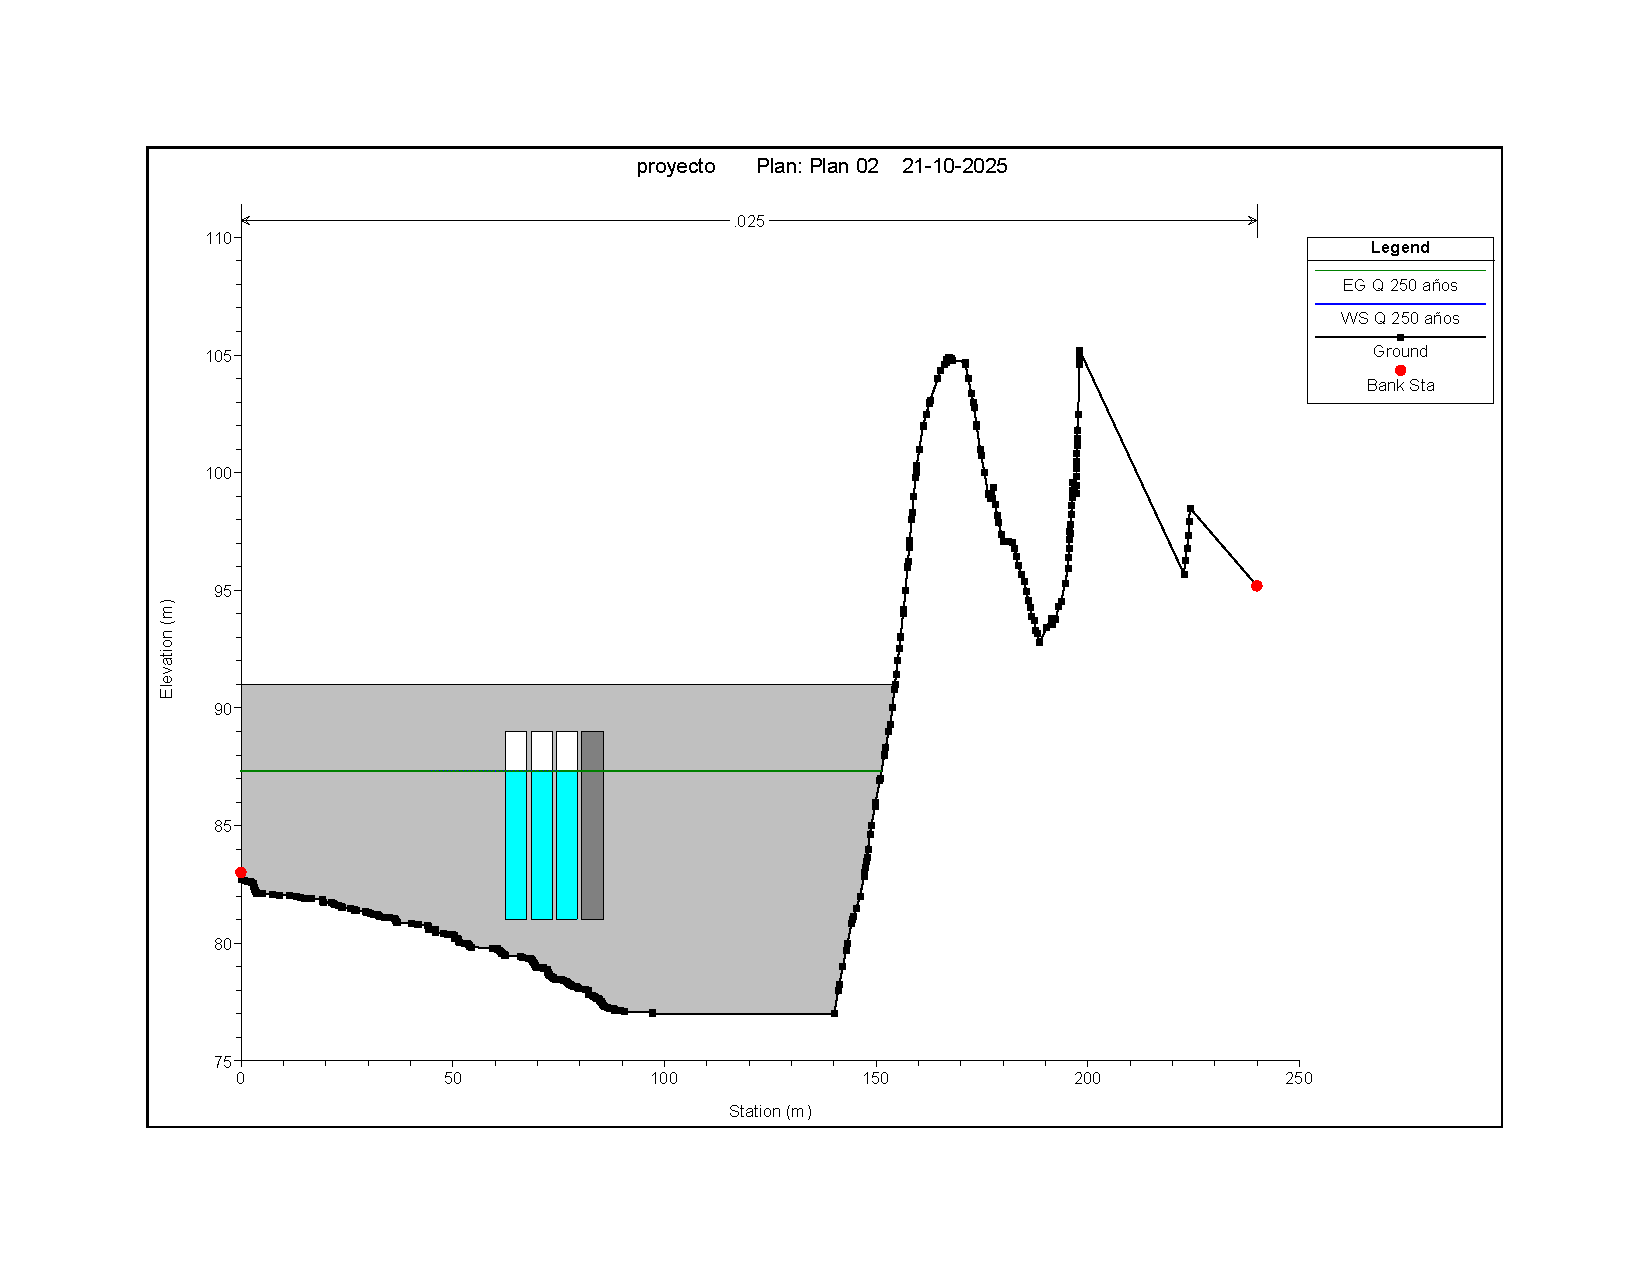
\includegraphics[width=0.6\linewidth]{imagenes/corte_250_cb.pdf}
    \caption{Corte transversal del río Pilmaiquén con muro y bocatomas para periodo de retorno de 250 años}
\end{figure}

\begin{figure}[H]
    \centering
    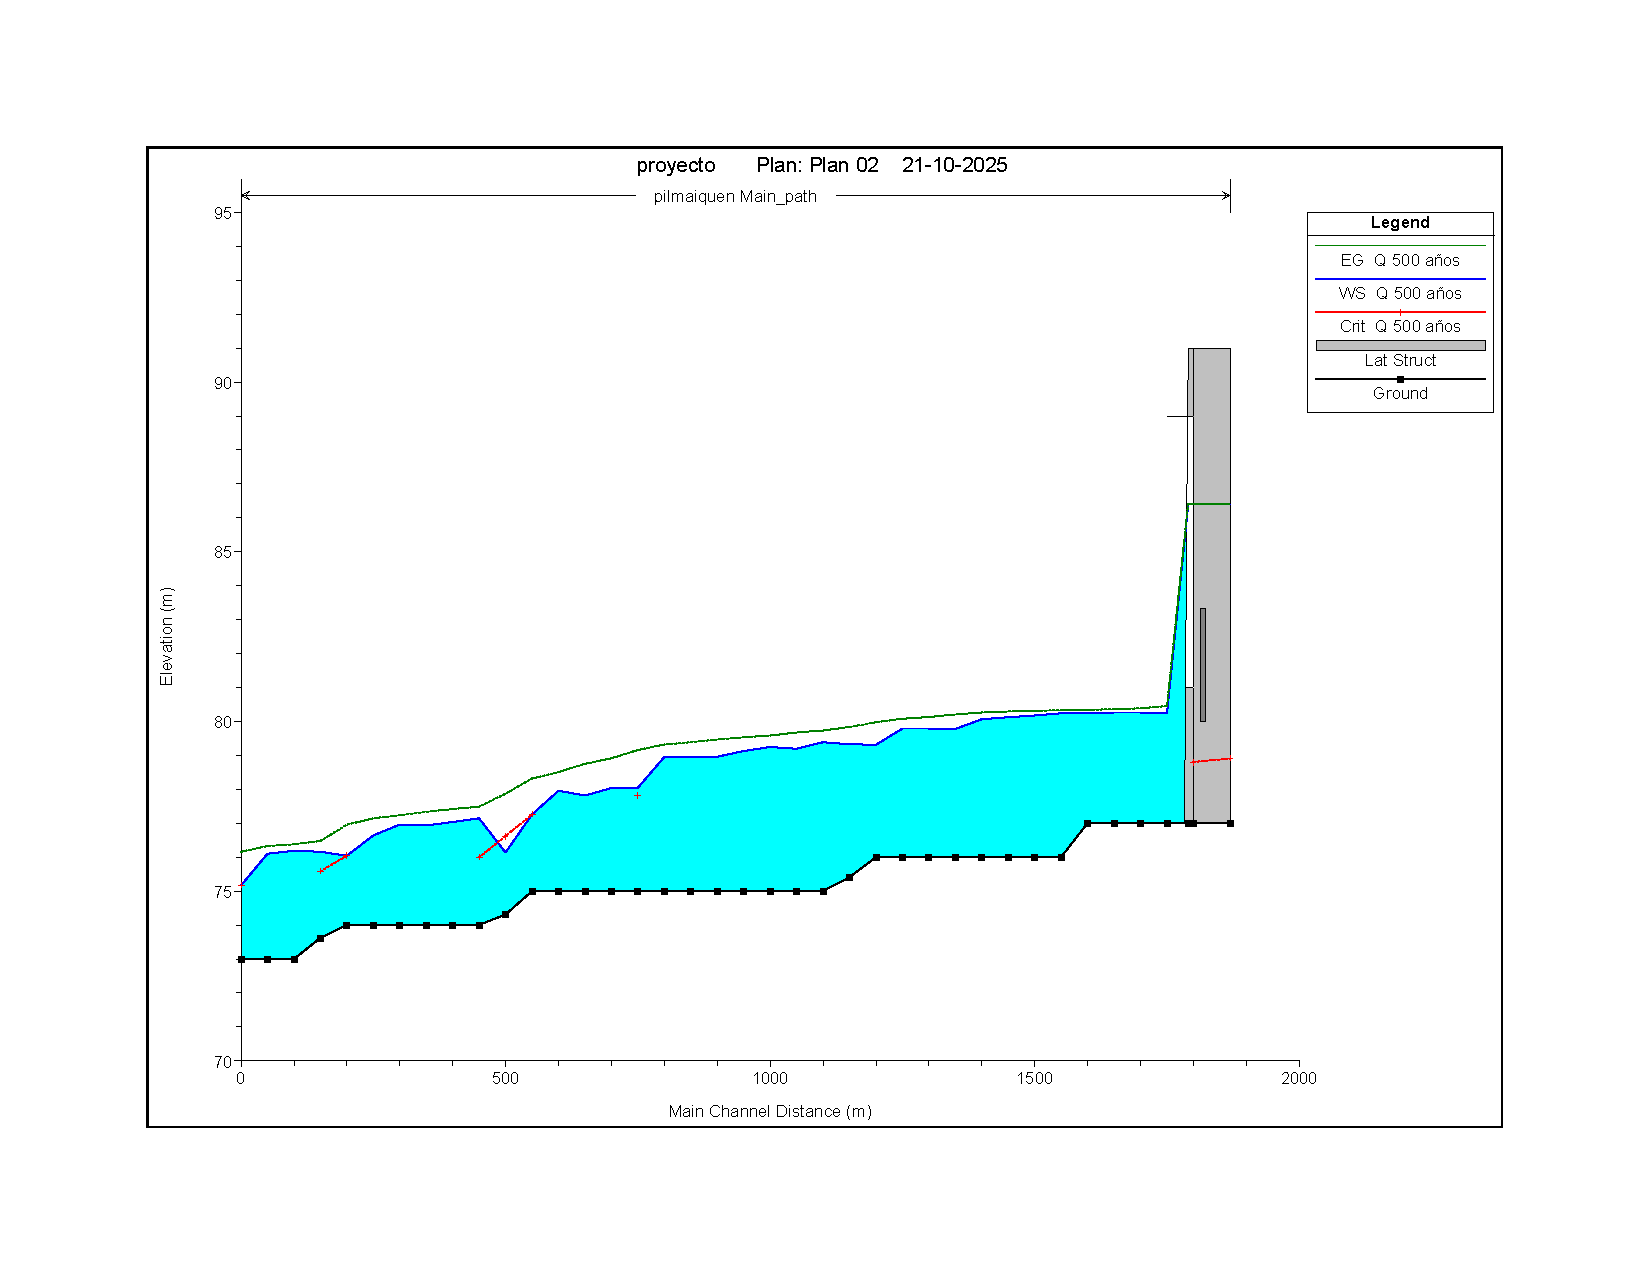
\includegraphics[width=0.6\linewidth]{imagenes/perfil_500_cb.pdf}
    \caption{Perfil hidráulico con caudal asociado a periodo de retorno de 500 años con muro y bocatomas}
\end{figure}

\begin{figure}[H]
    \centering
    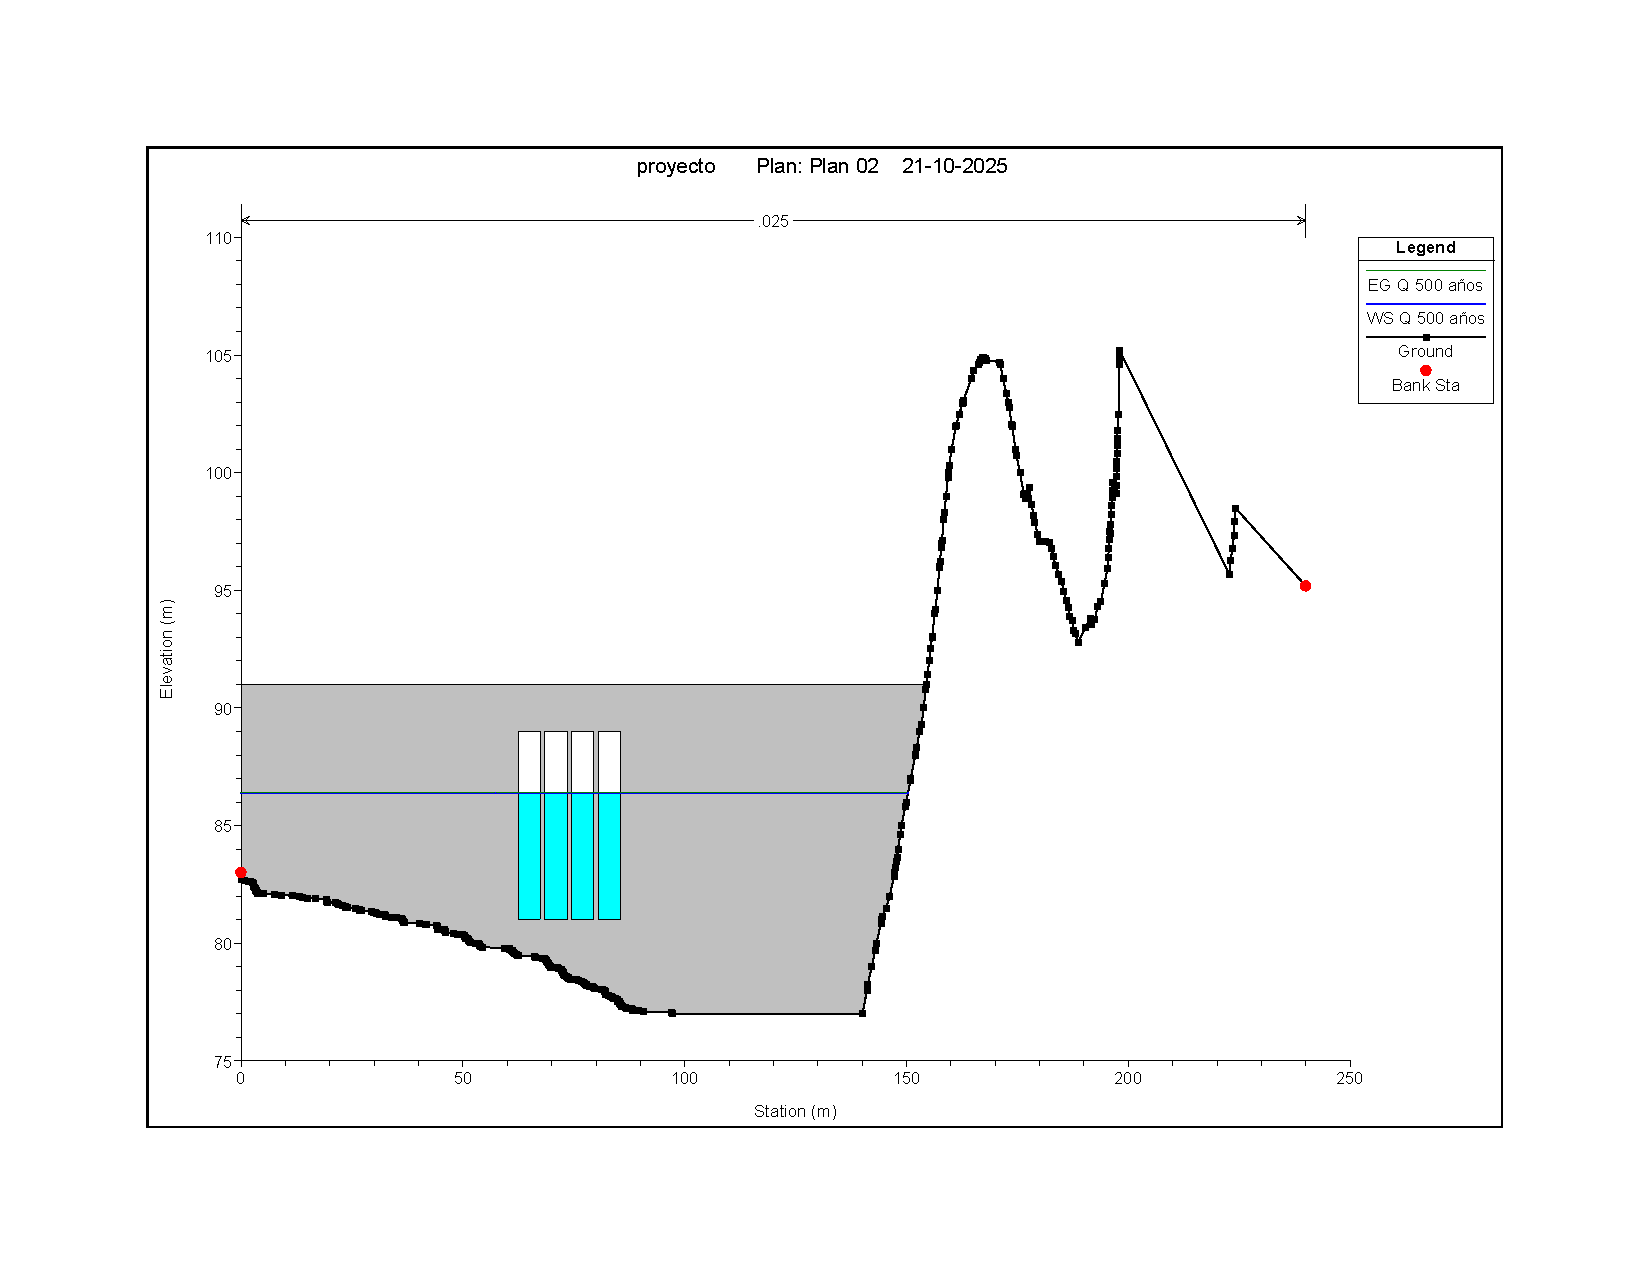
\includegraphics[width=0.6\linewidth]{imagenes/corte_500_cb.pdf}
    \caption{Corte transversal del río Pilmaiquén con muro y bocatomas para periodo de retorno de 500 años}
\end{figure}

\newpage
\section{Conclusiones}

El diseño desarrollado para la obra de captación y la barrera de derivación del río Pilmaiquén cumple con los objetivos hidráulicos, estructurales y operativos establecidos. Los resultados obtenidos demuestran que la propuesta permite derivar un caudal de 10 m³/s de forma segura, estable y controlada, asegurando la continuidad del servicio incluso bajo condiciones de crecida extrema.

El análisis hidráulico, complementado con las simulaciones en HEC-RAS, evidenció que las condiciones de flujo se mantienen dentro de los márgenes de estabilidad previstos, tanto para la crecida de diseño (250 años) como para la de verificación (500 años). La adopción de una barrera mixta —con un módulo de compuertas en concreto armado y un tramo en tierra compactada— resultó ser la alternativa más eficiente, al equilibrar resistencia estructural, estabilidad geotécnica y economía constructiva.

La altura crítica obtenida (\(B_c = 7{,}4\ \text{m}\)) determinó el dimensionamiento final de las compuertas, las cuales, con una altura de 8 m, incorporan la revancha necesaria para absorber variaciones del flujo y mantener un régimen estable. Asimismo, los taludes de 3H:1V aguas arriba y 2,5H:1V aguas abajo garantizan la estabilidad del terraplén ante las solicitaciones esperadas.

En conclusión, la obra propuesta cumple los criterios técnicos y normativos aplicables a una estructura de \textit{Categoría A}, ofreciendo una solución robusta y funcional. El sistema de captación planteado aprovecha de manera eficiente los recursos hídricos del río Pilmaiquén, asegurando su operación segura y sostenible en el tiempo.



\end{document}